%-----------------------------------------------------
% Chapter: Methodology
%-----------------------------------------------------
\chapter{Methodology}
This chapter describes the methodology used throughout the project as well as rational behind certain methodological decisions. 
\label{chap:data_methodology}
\section{Collecting Data}
As previously mentioned, a central repository for song lyrics, where downloading is permissive, is non-existent. Collection of song lyrics from sites such as Genius\footnote{https://genius.com/} is only achievable through web scraping: a process which involves the exhaustive downloading and processing of web pages from either a predefined list of URLs or the recursive process of link extraction and following (commonly known as \textit{web crawling}) from a given seed URL. When scraping at scale, restrictions such as the robots exclusion protocol, which specifies areas of a website that are allowed to be processed, and crawl rate, which specifies the minimum delay between requests, make data collection via this method a troublesome task. Taking into account the project aims and constraints such as time, web scraping was deemed unfavourable and hence avoided for data collection.

\noindent
\newline
To fulfil the data requirements of the project, a public dataset \footnote{https://www.kaggle.com/neisse/scrapped-lyrics-from-6-genres} containing over 250,000 song lyrics was used. The dataset, which was scraped from Brazilian music website Vagalume.br, comprised of two \textit{.csv} files: artists-data and lyrics-data. The artist-data file included metrics such as popularity, genre and number of songs per artist, whilst the lyrics-data file contained song lyrics for individual songs by artists.

\section{Data Analysis and Restructuring}
The CoVeR algorithm requires each document within a corpus to be associated with a covariate in order to jointly learn word embeddings and the relevant transformation matrices. To satisfy this requirement, Pandas, a Python data analysis library, was used to perform a join operation on the artists columns in both the artists-data and lyrics-data files. The result of this operation followed by the additional dropping of redundant columns resulted in the dataset used throughout the rest of the project.

\noindent
\newline
A trivial approach to divide the dataset on genre would involve an equal split for equal representation, however, this method has the assumption that for each genre, word count per song is equivalent. Examining the dataset however, proved this not to be the case.
\begin{figure}[h]
	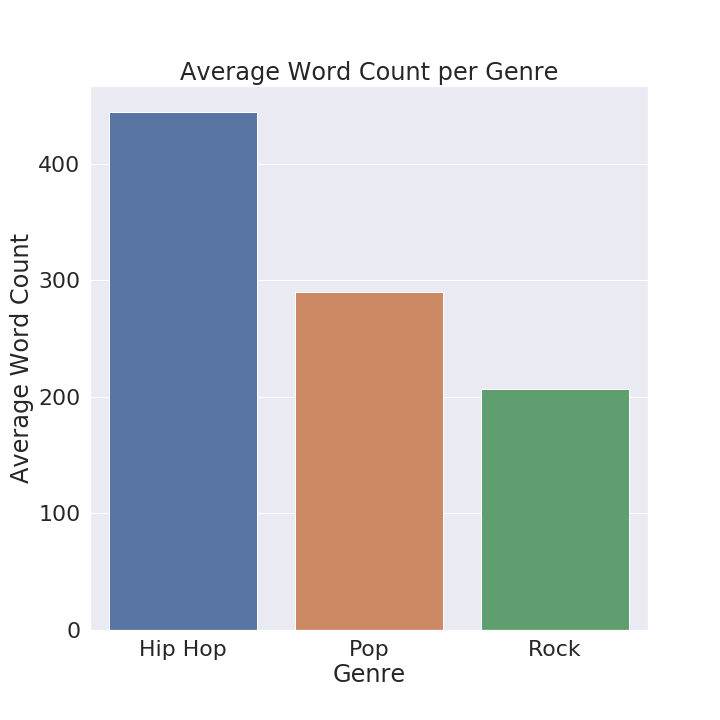
\includegraphics[width=8cm, height=8cm]{./figures/fig6}
	\centering
	\caption[Average Song Word Count by Genre]{Average song word count by genre for all lyrics within the dataset.}
	\label{fig:fig6}
\end{figure}

\noindent
\newline
Analysing the dataset, the mean number of words contained in a Hip Hop song was 444; being more than double the mean number of words found in Rock songs, which had a count of 207. With regards to the Pop, the mean word count per song was 289. To reflect these statistics and also due to constraints in the distribution of data by genre, 100,000 song lyrics were randomly selected to create the dataset to be used to train CoVeR. Moreover, a data split of 48:30:22 for Rock, Pop and Hip-Hop, was to maintain an even distribution of words by song genre within the dataset.
\section{Data Pre-processing}
Essential to any machine learning task is the pre-processing of input data in such a way that important features are accessible during training. In NLP, this can include techniques such as tokenisation, string cleaning, stemming and lemmatisation.

\noindent
\newline
Following reconstructing of the original dataset, each song lyric in the dataset was cleansed and tokenised. The following string cleaning techniques were applied to each song lyric.

\begin{enumerate}
	\item All characters, except for letters, were substituted with a space.
	\item All letters were lowercased.
	\item All text between curly and square brackets were removed. (This was to ensure text like \textbf{[Verse 1]} was not included during training).
	\item All trailing white space was removed.
\end{enumerate}

\noindent
\newline
Tokenisation is the process of separating textual inputs into meaningful chunks called \textit{tokens}. Naturally to create word embeddings, text is tokenised at the word level and each token is assigned a unique integer key to map the token to its future word embedding.

\section{Hyperparameters}
In machine learning hyperparameters are parameters that govern a given model. The selection of these parameters directly impacts the performance of a given training algorithm and as such, hyperparameter choice is important for producing optimal performance for a given model. Commonly, techniques such as grid search, random search and manual search are used to find optimal optimal parameters for a given training algorithm. However, due to project time constraints, hyperparameter search was limited.

\noindent
\newline
Both the CoVeR algorithm and LSTM networks have important hyperparameters which are reviewed in the following sections
\subsection{CoVeR Hyperparamters}
\subsubsection{Removing Rare Words}
Word embedding algorithms such as word2vec typically remove rare occurring words within a corpus before training takes place. In the case of word2vec, rare words are removed \textit{before} the computation of co-occurrence statistics. This method of removal has the effect of generating context windows differing to what would have been created if the corpus had remained intact. In turn, this produces different word co-occurrences and hence a different co-occurrence matrix. For example, applying a symmetric context window of size 1 over the following sentence

\begin{center}
	"We're gonna rock the night away"
\end{center}

\noindent
and assuming the focal word was \textit{"the"}, the original context words in this window would include \textit{"rock"} and \textit{"night"}. However, suppose the words \textit{"rock"} and \textit{"night"} were deemed as rarely occurring words and removed, the sentence above would then be processed as 

\begin{center}
	"We're gonna the away"
\end{center}
\noindent
and examining the same focal word as before, the new context words in this window become \textit{"gonna"} and \textit{"away"}.

\noindent
\newline
Neither the CoVeR or GloVe paper, discuss the explicit removal of rare words, however many implementations of GloVe, for the sake of computation, restrict the vocabulary of a corpus to the top \(N\) most words. For this project this number was 20,000.
\subsubsection{Subsampling}
Typically found within text corpora are high frequency stop words which provide less information than infrequent or domain specific words (\cite{Mikolov2013a}). For example, from a music related corpus, co-occurring examples of the words "king" and "pop" (referring to Michael Jackson), are more beneficial to a model then examples of co-occurring words "the" and "king". This is because "the" would co-occur with the majority of words within the corpus. This concept of oversaturated co-occurrences can also be applied to word embeddings; where the word embeddings of frequent words does not change significantly after training on several examples.
Existing methods for removing high frequency words involve the complete removal of stop-words during preprocessing, however, for the sake of this project, where the appearance of such words is necessary to create a language model, subsampling is used instead. Subsampling is the process of sampling infrequent words more often than frequently occurring words in order to create new training data. In the case of word embedding algorithms, subsampling increases training speed by randomly removing very frequent word co-occurrence which provide little to no extra benefit to the model. Taking inspiration from word2vec, subsampling was used at the covariate level using the following adapted formula from the original word2vec implementation.

\begin{equation}
P(w_{ik}) = \sqrt{\dfrac{z(w_{ik})}{t}} + 1 \cdot \dfrac{t}{z(w_{ik})}
\end{equation}

\noindent
\newline
where \(z(w_{ik})\) is the percentage of word \(w_{ik}\) in covariate \(k\) and \(t\) is a chosen threshold. For this project the threshold that worked well was 0.05.
\subsubsection{Context Windows}
CoVeR uses the same weighted context windows strategy as GloVe during the process of calculating co-occurrence statistics. During experiential training, a context window size of 8 is used in the paper however, the paper does not detail the type of context window used. Typically, context windows can either be asymmetric, where only preceding words are considered or symmetric, where words are considered on either side of a given focal word. An experimental finding in the original GloVe paper states that small and asymmetric context windows work well for syntactic tasks, whilst long and asymmetric tasks are good for semantic tasks. Relating back to one of the functional requirements, specifically requirement FR4, the resulting word embeddings will be used for a word suggestion feature, where suggested words correspond to the closest words in the embedding space. This requirement can be considered more of a semantic task than a syntactic task due the feature being synonymous with a thesauruses for the sake of providing words with similar meanings. For this reason, a symmetric context window is used for this project.
\subsubsection{Embedding Size}
Common embedding sizes for models such as GloVe and word2vec, range in dimensionality with typical values being between 50-300 dimensions. Currently there is no empirical method in selecting the dimension size for word embeddings. For this project, word similarity, discussed in \autoref{chap:evaluation} was an important measure to evaluate the semantic quality of the word embeddings. Dimensionality values 50, 100, 200 yielded similar results word similarity results as shown in \autoref{Tab:testembeddingdim}.

\begin{table}[htbp]
	\label{Tab:testembeddingdim}
	\begin{center}
		\begin{tabular}{|c|c|c|c|}
			\hline
			{Focal Word}& \multicolumn{3}{p{5cm}|}{\centering Number of Dimensions} \\
			\cline{2-4} & \multicolumn{1}{c|}{50} & \multicolumn{1}{c|}{100} & \multicolumn{1}{c|}{200} \\ \hline
			king & princess, queen, prince & queen, princess, hearts & queen, prince, hearts \\
			drink & pass, beer, bottle & drink, somebody, pass & bottle, pour, lets \\
			lord & praying, pray, child & knows, praying, please & knows, please, praying \\
			fire & burning, fireball, desire & fireball, burning, desire & fireball, burning, light \\
			\hline
		\end{tabular}
	\end{center}
	\caption[Word Similarity by Dimension]{Comparison of the three most similar words to multiple focal words by dimension. The differences between dimensions was minimal and as such 50 was the chosen dimension size to increase training speed.}
\end{table} 

\noindent
For the purpose of this project and to help speed up model training  for later tasks, an embedding dimension of size 50 was chosen for this project.
\subsubsection{Optimiser}
Similar to the GloVe method, the CoVeR algorithm utilises stochastic gradient descent to minimise its objective function. Rather than using Adagrad, CoVeR utilises the Adam optimiser (\cite{Kingma2014}). For this project the same optimiser is used to train the CoVeR embeddings.
\subsection{LSTM Hyperparameters}
Both the language model and text classifier used in this project take advantage of an LSTM. Structurally, both models are the same: making use of an embedding layer, a recurrent layer, and a dense layer with a softmax activation function to help it predict the probaiilty distributioon. The general architetcure of both models can be seen below in ...  
\subsubsection{Dropout}
Dropout is a regularization technique proposed by \cite{Srivastava2014}, which involves the random dropping of neurons and their connections within a network, omitting them during a particular forward or backward pass. Selected neurons are picked at random using a probability known as the dropout rate. Dropout helps to decrease over-fitting as it prevents neurons from co-depending on one another as they must learn to work with a random sample of other neurons rather than the same fixed ones. This in turn forces the neuron to learn useful connections rather than relying on other neurons for correction. As utilised in \cite{Srivastava2014}, dropout is applied at both the input and hidden layers, with a rate of 0.2 and 0.5 respectively.
\subsubsection{Embedding Layer}
For both the language model and the text classifier, the input layer to the network is the embedding layer which transforms words, represented as indices, into word embeddings. These embeddings can either be initialised randomly as one-hot vectors and trained with the network or they can be initialised using pre trained word embeddings, which can either be left as is or trained further. For this project the word embeddings derived from CoVeR were used as the weight initialiser for the embedding layer, and were not allowed to be trained. The motivation behind this was to see how well the genre specific word embeddings contributed towards creating genre specific language models, as well as how well they contributed towards the task of binary text classification, discussed in \autoref{chap:evaluation}.
\subsubsection{Optimiser}

